
\begin{titlepage}

	%\begin{tikzpicture}[remember picture,overlay] \node[opacity=0.15,inner sep=0pt] at (current page.center){\includegraphics[width=\paperwidth,height=\paperheight]{Pictures/wave_wall_paper2.png}};
    %\end{tikzpicture}

	\begin{center}

	{\Huge{\bfseries{Notes on Quiver Gauge Theories}}}\\[0.7cm]

	Louan Mol - \textit{Université Libre de Bruxelles}

    \vspace{1cm}

	\begin{figure}[H]
        \centering
        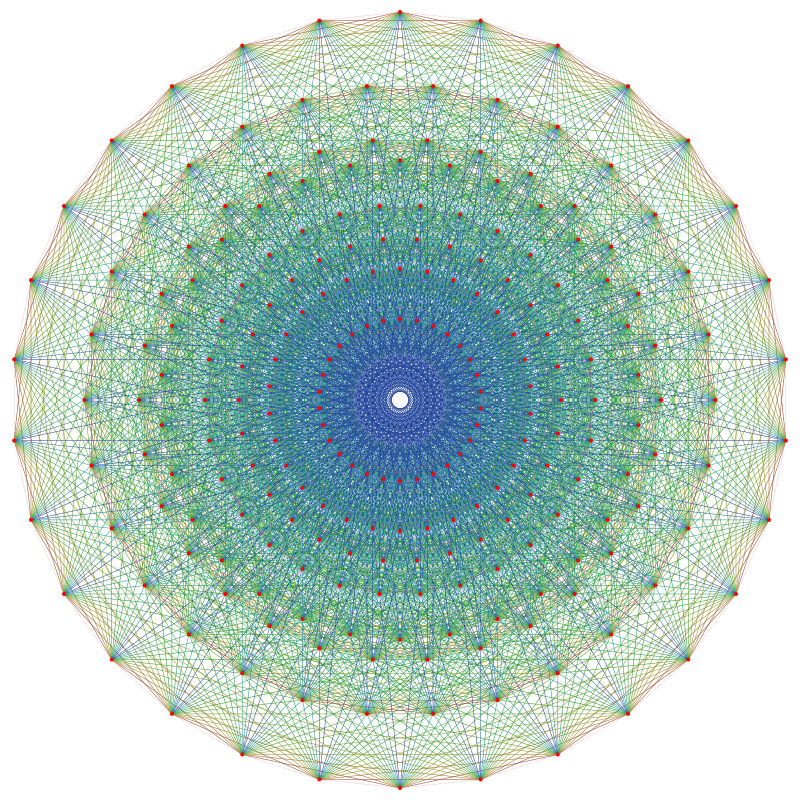
\includegraphics[scale=0.4]{Pictures/E8_graph.png}
    \end{figure}

    \vspace{2cm}
	
	{\large\textbf{Abstract}}
	\end{center}
	
	    \quad In these notes, we present some basic ideas around the large topic of quiver gauge theories, more precisely about their brane probes construction.  The goal is to reproduce and regroup the basics of these theories for various types of singularities, with increasing level of complexity (orbifold, toric, del Pezzo, etc). Note that this document is only meant as a work support and contains a lot of typos, errors and imprecisions.
	    
	\vfill

	Last update on \today.
	
\end{titlepage}